\chapter{先行研究}
本章では,本研究における先行研究を述べる.

\section{概要}
林ら\cite{biblabel1}は,バーチャルペットと比較して実体を有するペットロボットの方がセラピー効果が高いと考え,ふれあいによる心理・生理的なストレスの緩和効果の差異を比較・検証を行った.

検証に使用するペットロボットは,林らが開発した柔らかい触感を有するセラピーロボット「ちょぼにゃん」である.頭部に配置された接触を検知するセンサ部,人工筋肉でできた尻尾に位置する感情表出部,感情表出部を制御する制御部から構成されている.
バーチャルペットは「ちょぼにゃん」を模した3DCGキャラクタの「ちょじにゃん」が林らにより開発され,実験に用いられた.「ちょじにゃん」はユーザの接触動作をペットロボットに出来る限り近付けるために,Leap Motionを用いる.これによりトラッキングされた手の位置は仮想ハンドとして画面上に反映され,ちょじにゃんへの頭を撫でる,叩くといったユーザの接触を検知できる.

\begin{figure}[H]
\centering
\begin{tabular}{c}

\begin{minipage}{0.50\hsize}
\includegraphics*[width=8.5cm,clip]{images/先行研究1.eps}
\caption{ちょぼにゃんの外観}
\label{fig:system1}
\end{minipage}

\begin{minipage}{0.50\hsize}
\centering
\includegraphics*[width=8.5cm,clip]{images/先行研究2.eps}
\caption{ちょじにゃんの外観}
\label{fig:system2}
\end{minipage}

\end{tabular}
\end{figure} 

ペットロボット,バーチャルペット共にユーザが頭を撫でた時は尻尾を左右に振り喜びを表現を,ユーザが頭を叩いた時には尻尾を垂れ下げ悲しみ表現を表出するといった二種類の反応行動を行う.
\newpage

\begin{figure}[H]
\centering
\includegraphics*[width=8.5cm,clip]{images/先行研究3.eps}
\caption{反応行動}
\label{fig:system3}
\end{figure} 

バーチャルペットとペットロボットのセラピー効果を比較するため,心理的,生理的の二面からストレス緩和効果の比較検証実験を行った.
心理効果の評価実験では,まず実験参加者にストレスを与えるために,被験者に計算課題を2分間行った.計算課題終了後,POMSと呼ばれる気分プロフィール検査を実施した.
質問用紙を回収後にペットロボット,もしくはバーチャルペットと2分間自由にふれあってもらい,再度POMS検査を行った.最後に,ふれあったペットの印象の評価としてSD尺度法を用いて回答を求めた.
実験の結果,ペットロボットとバーチャルペットともに心理的なストレス緩和効果があることが分かった.
特にペットロボットはバーチャルペットと比較して有意な変化が認められた尺度が多く,特に緊張の緩和効果と活気の尺度において高い効果を示した.
親密性ではペットロボットの方で高い値が確認されたが,力本性と信頼性においてはバーチャルペットの方が高い.以上より,ペットロボットとバーチャルペットが与える印象の性質に差があると記述している.

生理的効果の評価実験では,心理的効果測定と同様にまず計算課題を実施する.その後,MindWave Mobileを用いて被験者の安静閉眼時の脳の状態を1分間計測した.MindWave Mobileとは,国際10-20法のFp1領域の脳波を計測可能な簡易脳波計である.
次に,ペットロボット,もしくはバーチャルペットと2分間ふれあってもらい,その後再度被験者の安静閉眼時の脳状態を1分間計測した.
実験の結果,ペットロボットにはα波の含有率の増加,β波の減少が確認された.α波はリラックスしている時に,β波は精神的に緊張しているときに多く出現するとされている.一方バーチャルペットには,α派,β波共に変化が殆ど確認できなかった.
このことから,ペットロボットは生理的なストレス緩和効果を持つが,バーチャルペットは持たないということが分かった.

以上二つの評価実験の結果から,生理的,心理的どちらの側面においてもペットロボットの方が高いストレス緩和効果を得ることができた.検証した全ての比較結果を下の表に示す.

\begin{table}[H]
\centering
\label{table:cal}
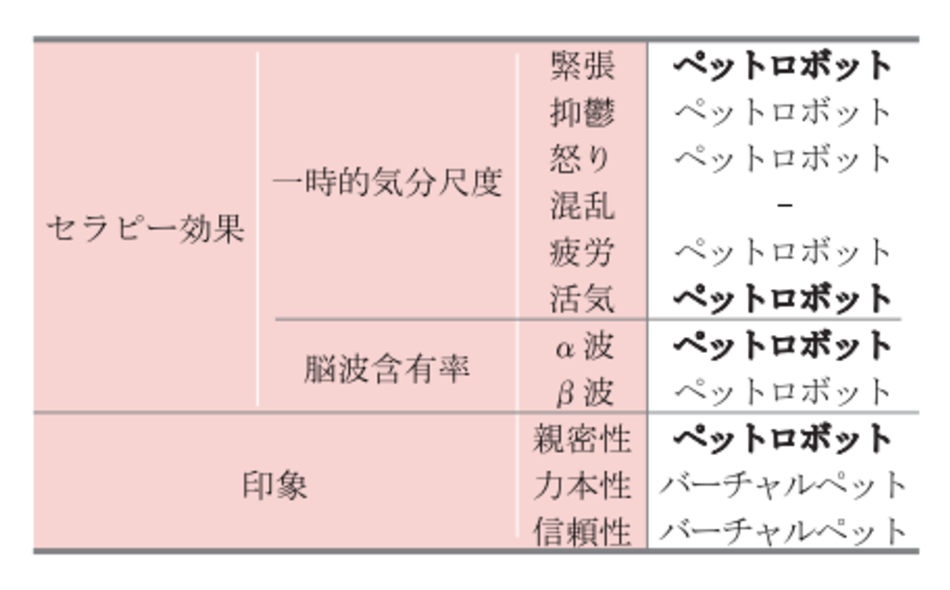
\includegraphics[width=8cm]{images/先行研究6.eps}
\caption{ペットロボットとバーチャルペットの比較}
\end{table}

このような結果になった要因として,林らは「接触フィードバック」「現実感」という二点のキーワードをあげている.
まず,接触フィードバックとはユーザの接触に対するペットからのフィードバックのことである.ペットロボットは現実に存在しているために,接触すれば感触がそのまま返ってくる.しかしながら,バーチャルペットは実在しないために感触が返ってくることがない.実験参加者の9割が,自身の手が接触しているのかどうか分かりづらく,戸惑ったと答えている.林らは接触フィードバックは身体性が持つ特性の一つであると記述している.
次に現実感について,実験に使用されたバーチャルペットはタブレット上に表示された3DCGキャラクタであり,このことから実験参加者の8割がゲームで遊んでいるような感覚だったと答えた.一方ペットロボットとのふれあいにおいては,実験参加者の7割が動物と接している感覚に近く,親しみやすかったと答えた.現実感についても身体性が持つ特性の一つであると記述している.

\section{問題点}
林らはペットロボットと比較して,バーチャルペットは身体性を有さないためにセラピー効果が低いとしている.
しかしながら,バーチャルペットにおいても利用技術によって身体性を付与することは可能であると考える.
本研究では,ヘッドマウントディスプレイを用いて360度全方位に映像を出力することで疑似的な現実感をユーザに与え,更にコントローラの振動を利用して接触フィードバックを実装した身体性を有するバーチャルペットの開発を行う.
